\chapter{线性代数}
\label{ch:linear_algebra}

线性代数是广泛使用在整个科学和工程中的一个数学分支。然而,由于线性代数是一种连续
的形式而不是离散数学,许多计算机科学家对它少有经验。很好地理解线性代数,对理解和
使用许多\gls*{ml}算法来工作,是必不可少的,对\gls*{dl}尤其如此。因此,我们在介
绍\gls*{dl}之前先专注于对关键的线性代数必备知识做些陈述。

如果你已经熟悉了线性代数,尽管跳过这一章。如果你对这些概念有了一些先期的经验,但
是需要一个详细的参考来复习关键的公式,我们推荐 \emph{The Matrix Cookbook}
\citep{matrix-cookbook}。如果你完全没有接触过线性代数,这一章会教你足够的知识来阅
读本书,但是我们强烈建议你也去咨询其它专门教授线性代数的材料,例
如\citep{shilov1977linear}。本章会完全略过很多重要的线性代数的主题,它们对理
解\gls*{dl}不是必须的。

\section{标量、向量、矩阵和张量}
\label{scalars_vectors_matrices_and_tensors}

线性代数的研究涉及到几种数学对象的类型:

\begin{itemize}
\item \emph{\gls{scalars}}:一个\gls*{scalar}仅仅是一个单独的数字,相反,大多数其
  它线性代数的研究对象通常是多个数字排列。我们用斜体来写\gls*{scalar}。我们通常用
  小写命名\gls*{scalar}。当我们介绍它们时,我们指定它们是什么样的数字。例如:当定
  义一个实数值的\gls*{scalar}时,我们可能说``设 $s \in \mathbb{R}$ 为直线的斜率'',
  或者,当定义一个自然数\gls*{scalar}时,``设 $n \in \mathbb{N}$ 为单元的个数''。
\item \emph{\gls{vectors}}:一个\gls*{vector}是数字的一种排列。这些数字按照顺序排
  列。我们可以通过这一顺序中的索引来确定每一个单独的数字。通常我们以小写的粗体字
  体给\gls*{vector}命名,例如 $\pmb{x}$。\gls*{vector}的元素以伴有下标的斜体字体
  表示。$\pmb{x}$ 的第一个元素是
  $x_1$,第二个是$x_2$,依此类推。我们还要说明\gls*{vector}中存储的是什么类型的数
  字。如果每个元素是 $\mathbb{R}$ 中的数,而\gls*{vector}有 $n$ 个元素,那
  么\gls*{vector}位于以 $\mathbb{R}$ 的 $n$ 次笛卡尔积的所形成的集合内,表示
  为$\mathbb{R}^n$。当我们需要显示地表示一个\gls*{vector}中的元素,我们把它们写成
  方括号围起来的一列:
  \begin{equation}
    x = \begin{bmatrix}x_1\\ x_2\\ \vdots\\ x_n\end{bmatrix}
    \label{eq:vector_example}
  \end{equation}
  我们可以把\gls*{vector}看做表示空间的点,每个元素提供沿着不同坐标轴的坐标。\\
  有时候我们需要索引一个向量中的一个元素集合。在这种情况下,我们定义一个包含索引
  的集合,并把这个集合写成一个下标。例如,为了获得 $x_1$,$x_3$ 和 $x_6$,我们定
  义集合 $S = {1, 3, 6}$,写为 $\pmb{x}_S$。我们使用 $-$ 标记表示一个集合的补充。
  例如 $\pmb{x}_{-1}$ 是包含 $\pmb{x}$ 中除了 $x_1$ 的所有元素
  的\gls*{vector},而 $\pmb{x}_{-S}$ 是包含 $\pmb{x}$ 中除
  了 $x_1$,$x_2$ 和 $x_6$ 之外的所有元素的向量。
\item \emph{\gls{matrices}}:一个矩阵是一个数字的二维数组,所以每个元素由两个索引
  确定,而不是一个。我们通常用大写的粗体字体表示矩阵,例如 $\pmb{A}$。如果一个实
  数值的矩阵 $\pmb{A}$ 高度为 $m$,宽度为 $n$,那么我们说
  $\pmb{A} \in \mathbb{R}^{m \times n}$。我们通常使用斜体~——~但不是粗体字体~——~表
  示一个矩阵的元素,索引用逗号分开列出。例如,$A_{1,1}$ 是 $\pmb{A}$ 左上角的元素,
  而 $A_{m,n}$ 是右下角的元素。我们可以为横向坐标写一个 ``:'' 来表示所有竖向坐
  标 $i$ 的数字。例如,$\pmb{A}_{i,:}$ 表示竖向坐标 $i$ 的横跨 $\pmb{A}$ 的部分。
  即 $\pmb{A}$ 的第 $i$ 行。同样的,$\pmb{A}_{:,i}$ 是 $\pmb{A}$ 的第 $i$ 列。当
  我们需要显式地表示一个矩阵的元素,我们把它们写成一个用方括号围起来的数组:
  \begin{equation}
    \begin{bmatrix}A_{1,1} & A_{1,2} \\ A_{2,1} & A_{2,2}\end{bmatrix}
    \label{eq:matrix_example}
  \end{equation}
  有时候我们可能需要索引矩阵值的表达式,它不仅仅是一个单个的字母。在这种情况下,
  我们在表达式后使用下标,但不转换为小写。例如,$f(\pmb{A})_{i,j}$ 给出了应用函
  数 $f$ 到 $\pmb{A}$ 上后计算得到的 $(i,j)$ 位置的元素。。
\item \emph{\gls{tensors}}:在有些情况下我们会需要一个多于两个坐标的数组。在一般
  情况下,排列在一个规则的网格~——~具有可变数量的坐标轴~——~上的数组,被称为一
  个\emph{\gls{tensor}}。我们用这样的字体表示一个名为 ``A'' 的张
  量:$\pmb{\mathsf{A}}$。我们把表示 $\pmb{\mathsf{A}}$ 在 $(i,j,k)$ 坐标的元素写
  为 $\mathsfit{A}_{i,j,k}$。
\end{itemize}

矩阵的一个重要的操作是\emph{\gls{transpose}}。一个矩阵的\gls*{transpose}是将矩阵
沿着一个对角线~——~称为\emph{\gls{main-diag}},从左上角指向右下角~——~做镜像。参见
图~\ref{fig:transpose_of_matrix} 中对这个操作的图形化描述。我们把一个矩
阵 $\pmb{A}$ 的转置表示为 $\pmb{A}^{\top}$,以这样定义
\begin{equation}
  (\pmb{A}^{\top})_{i,j} = A_{j,i}
  \label{eq:transpose_of_matrix}
\end{equation}

\begin{figure}[h]
  \centering
  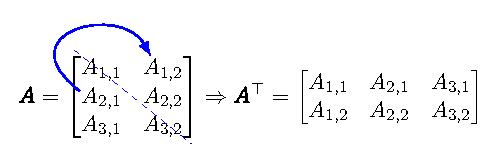
\includegraphics{transpose_of_matrix}
  \caption{矩阵的转置可以被看做沿着\gls*{main-diag}的镜
    像\label{fig:transpose_of_matrix}}
\end{figure}

\section{矩阵和向量的乘法法则}
\label{sec:multiplying_matrices_and_vectors}

